\documentclass[11pt]{article}
\usepackage[margin=1in]{geometry}
\usepackage[T1]{fontenc}
\usepackage{enumitem}
\usepackage{xurl}
\usepackage{hyperref}
\usepackage{longtable}
\usepackage{array}
\usepackage{booktabs}
\usepackage{tikz}
\usepackage{float}
\hypersetup{colorlinks=true,urlcolor=blue,linkcolor=blue}
\setlist{nosep,leftmargin=*}

\title{Final Project: Tracing and Verifying AI Agent Tool Calls}
\author{Team project: two students per team}
\date{}
\begin{document}
\maketitle

\section{Project Overview}
Build a system that captures, reconstructs, visualizes, and verifies the tool-calling behavior of an AI agent. Use \textbf{Hermes Agent} or \textbf{OpenClaw} as the agent platform. Your system must show which tool calls actually occurred when an agent answered a question, their order or causal relationships, and their outcomes. The project is an implementation and evaluation task, not merely a diagram of an intended workflow.

Work in a team of exactly two students. Both students are responsible for understanding the entire system, testing it, writing the report, and presenting it. Teams receive the same project score when their documented contributions are substantially equal. The instructor may assign different individual scores when evidence shows unequal contributions.

\section{Required Outputs at a Glance}
\begin{enumerate}
  \item Run five required cases: M0--M2 again, plus F1 and F2. Add a run if none shows at least two actual tool calls.
  \item Use one documented command to turn each saved run and reference record into a machine-readable graph, a readable visualization, and a validation report.
  \item Check every graph against independent execution evidence; show that the validator detects a deliberately altered graph.
  \item Submit the IEEE report, editable Overleaf link, slides, and reproducible GitHub repository as described below.
\end{enumerate}

\section{Learning Objectives}
By the end of the project, you should be able to:
\begin{enumerate}
  \item Explain where tool calls occur in an agent run and what evidence is available to observe them.
  \item Design and implement a reproducible trace capture and graph construction method.
  \item Distinguish observed call order from inferred causal or data dependencies.
  \item Evaluate graph completeness and correctness against an independent source of evidence.
  \item Communicate the design, results, limitations, and team contributions in an IEEE-style report and presentation.
\end{enumerate}

\section{Platform and Project Scope}
Choose \textbf{one} platform: Hermes Agent (Nous Research) or OpenClaw. Record the installed version or commit, model/provider, operating environment, tool configuration, and tracing interface used. Use real agent executions. A hand-written list of expected calls or a simulated graph alone does not satisfy the implementation requirement. A deterministic mock tool is allowed for a controlled test, but the selected agent must actually invoke it.

Begin with official platform documentation and identify a supported observation point. For example, Hermes documents \texttt{pre\_tool\_call} and \texttt{post\_tool\_call} hooks; OpenClaw documents trajectory bundles, audit records, and OpenTelemetry signals. These are examples, not required implementation choices. Explain the coverage and limitations of the interface you choose. If it omits a type of tool action, supplement it with another observable source and document the reconciliation rule. Official starting points appear in Section~\ref{sec:sources}.

\section{Shared Starter Dataset and Questions}
Use the synthetic files and questions in \path{../tooltracking_starter/README.md}. Copy its \path{data/} folder into your controlled workspace and include the same files in your GitHub repository. \textbf{Rerun M0--M2 as new agent runs} using the same question wording as the midterm's first attempt, with \texttt{DATA\_DIR} replaced by the current path. Also run \textbf{F1 and F2} at least once. F0 and F3 are optional examples. These five required cases cover a no-tool control, simple and cross-file lookups, a three-source investigation, and a missing-file case. Add further runs or your own questions when the required cases do not elicit two actual tool calls or another required behavior. Document all prompt revisions. Compare midterm and final observations where useful, but do not assume the same prompt yields the same calls twice. Validate each final graph against its own independent execution record, not the answer key, the agent's narrative, or a saved midterm trace.

\subsection*{Illustrative tool-call graphs}
Figure~\ref{fig:example-calls} shows possible graph shapes for the required tests and a retry. Each box represents a separate \emph{observed} tool invocation, even when the same tool is called again. Arrows in this example mean \emph{next observed call in this run}; they do not claim that one call caused another. The question and final answer can appear in the graph caption or accompanying run record. These are examples only: a real agent may combine file reads into one call, repeat a call, or choose a different order. Your graph must reflect the actual saved run.

\begin{figure}[ht]
\centering
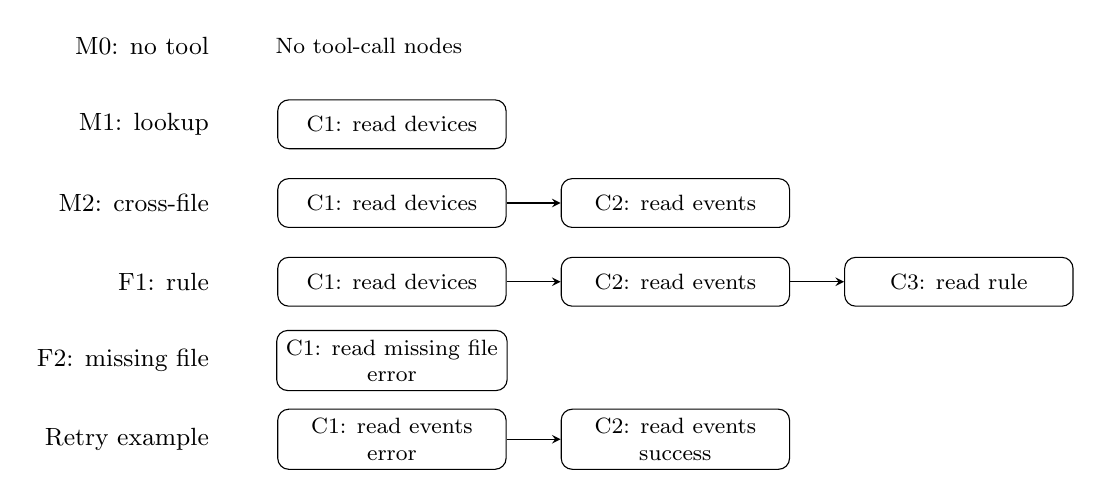
\begin{tikzpicture}[>=stealth,call/.style={draw,rounded corners,minimum width=2.9cm,minimum height=0.62cm,align=center,font=\footnotesize},row/.style={anchor=east,font=\small}]
  \node[row] at (2.5,0) {M0: no tool};
  \node[font=\footnotesize,anchor=west] at (3.1,0) {No tool-call nodes};
  \node[row] at (2.5,-1.0) {M1: lookup};
  \node[call] at (4.7,-1.0) {C1: read devices};
  \node[row] at (2.5,-2.0) {M2: cross-file};
  \node[call] (m2a) at (4.7,-2.0) {C1: read devices};
  \node[call] (m2b) at (8.3,-2.0) {C2: read events};
  \draw[->] (m2a) -- (m2b);
  \node[row] at (2.5,-3.0) {F1: rule};
  \node[call] (f1a) at (4.7,-3.0) {C1: read devices};
  \node[call] (f1b) at (8.3,-3.0) {C2: read events};
  \node[call] (f1c) at (11.9,-3.0) {C3: read rule};
  \draw[->] (f1a) -- (f1b);
  \draw[->] (f1b) -- (f1c);
  \node[row] at (2.5,-4.0) {F2: missing file};
  \node[call] at (4.7,-4.0) {C1: read missing file\\error};
  \node[row] at (2.5,-5.0) {Retry example};
  \node[call] (retry1) at (4.7,-5.0) {C1: read events\\error};
  \node[call] (retry2) at (8.3,-5.0) {C2: read events\\success};
  \draw[->] (retry1) -- (retry2);
\end{tikzpicture}
\caption{Illustrative call graphs. The retry uses two distinct nodes for the same tool; it is not a required outcome for F1 or F2. A refused F2 request could have no tool-call node.}
\label{fig:example-calls}
\end{figure}

\subsection*{Fictional branching investigation}
Consider the question: \emph{Which device owner, if any, meets alert rule R-1?} Imagine an agent with five example tools: \texttt{read\_auth\_events}, \texttt{read\_alert\_rule}, \texttt{read\_devices}, \texttt{evaluate\_rule}, and \texttt{match\_owner}. These tool names and the run in Figure~\ref{fig:dependency-example} are fictional teaching examples; they are not built-in Hermes or OpenClaw tools and are not an additional required test.

In this hypothetical run, C1 reads the events, C2 reads the rule, and C3 reads the device records. C4 uses the outputs of C1 and C2 to evaluate the rule. C5 uses the output of C4 and the device records from C3 to identify the owner. Each arrow in Figure~\ref{fig:dependency-example} means \emph{output used as input}, not next observed call. The three reads could occur in any order; the arrows do not establish parallel execution.

\begin{figure}[ht]
\centering
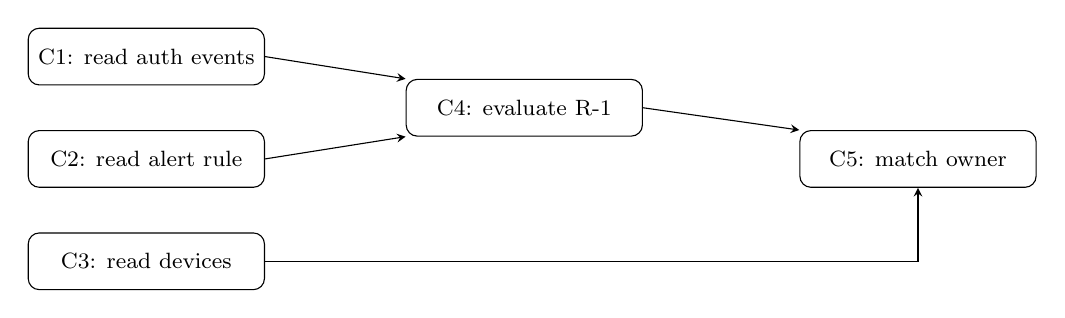
\begin{tikzpicture}[>=stealth,depnode/.style={draw,rounded corners,minimum width=3.0cm,minimum height=0.72cm,align=center,font=\footnotesize}]
  \node[depnode] (c1) at (2.2,0) {C1: read auth events};
  \node[depnode] (c2) at (2.2,-1.3) {C2: read alert rule};
  \node[depnode] (c3) at (2.2,-2.6) {C3: read devices};
  \node[depnode] (c4) at (7.0,-0.65) {C4: evaluate R-1};
  \node[depnode] (c5) at (12.0,-1.3) {C5: match owner};
  \draw[->] (c1.east) -- (c4.north west);
  \draw[->] (c2.east) -- (c4.south west);
  \draw[->] (c4.east) -- (c5.north west);
  \draw[->] (c3.east) -| (c5.south);
\end{tikzpicture}
\caption{Hypothetical data-dependency graph. Its branching shape is not required of student runs. Show a dependency edge only when evidence establishes that one call's output was used by another.}
\label{fig:dependency-example}
\end{figure}

This example shows why a complex tool-call graph can have branches and joins. A linear graph is also correct when that is what the observed calls and supported relationships show. Do not add dependency edges merely because a workflow diagram suggests them.

\clearpage
\subsection*{Fictional retry loop and write step}
Suppose the first event query returns too few records to decide whether R-1 applies. In an example workflow, an \texttt{evaluate\_rule} tool reports missing evidence, the agent calls \texttt{read\_auth\_events} again with a wider time window, evaluates the rule again, and then uses a fictional \texttt{write\_report} tool to save the conclusion in a disposable workspace. These are illustrative tool choices, not required tools or an additional graded case.

Figure~\ref{fig:loop-example} distinguishes a \emph{workflow loop} from the graph of actual call instances. The dashed arrow in the top panel means the agent may return to the read step when evidence is incomplete. The lower panel unrolls one possible run: C1 and C3 call the same read tool, but they are different invocations. Its solid arrows mean \emph{next observed call}, as in Figure~\ref{fig:example-calls}. A real graph must use the observed calls and supported edge relationships; it must not draw a self-loop on one invocation merely because the tool was used again.

\begin{figure}[H]
\centering
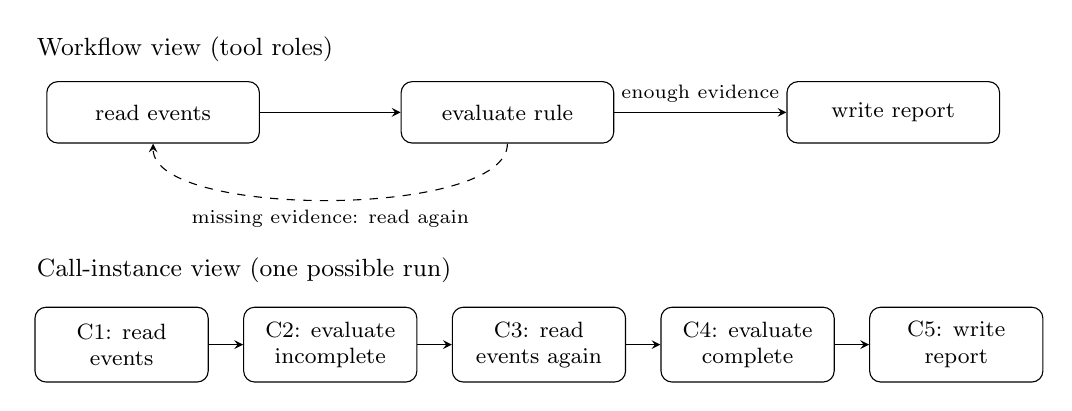
\begin{tikzpicture}[>=stealth,loopbox/.style={draw,rounded corners,minimum width=2.7cm,minimum height=0.78cm,align=center,font=\footnotesize},instance/.style={draw,rounded corners,minimum width=2.2cm,minimum height=0.95cm,align=center,font=\footnotesize}]
  \node[font=\small,anchor=west] at (0,0.8) {Workflow view (tool roles)};
  \node[loopbox] (read) at (1.6,0) {read events};
  \node[loopbox] (evaluate) at (6.1,0) {evaluate rule};
  \node[loopbox] (write) at (11.0,0) {write report};
  \draw[->] (read) -- (evaluate);
  \draw[->] (evaluate) -- node[above,font=\scriptsize] {enough evidence} (write);
  \draw[->,dashed] (evaluate.south) .. controls (6.1,-1.35) and (1.6,-1.35) .. node[below,font=\scriptsize] {missing evidence: read again} (read.south);
  \node[font=\small,anchor=west] at (0,-2.0) {Call-instance view (one possible run)};
  \node[instance] (c1) at (1.2,-2.95) {C1: read\\events};
  \node[instance] (c2) at (3.85,-2.95) {C2: evaluate\\incomplete};
  \node[instance] (c3) at (6.5,-2.95) {C3: read\\events again};
  \node[instance] (c4) at (9.15,-2.95) {C4: evaluate\\complete};
  \node[instance] (c5) at (11.8,-2.95) {C5: write\\report};
  \draw[->] (c1) -- (c2);
  \draw[->] (c2) -- (c3);
  \draw[->] (c3) -- (c4);
  \draw[->] (c4) -- (c5);
\end{tikzpicture}
\caption{A conceptual workflow loop (top) and one possible sequence of distinct tool-call instances (bottom). The write tool is fictional and is not required for student implementations.}
\label{fig:loop-example}
\end{figure}

\section{Required Technical Work}
\subsection{Propose a tracing solution}
Describe the problem, proposed architecture, alternatives considered, and why you selected your capture method. Include a data-flow diagram from agent event to stored trace, graph, and validation result. Define the trace boundary: one prompt, one run, one session, or another explicit unit. Specify what constitutes a tool call and whether failed, blocked, retried, nested, or parallel calls are included.

\subsection{Implement trace capture and graph construction}
Implement a runnable collector or parser and a graph generator. Preserve enough metadata to distinguish repeated calls to the same tool: at minimum a run identifier, unique call identifier (native or generated), tool name, event order or timestamp, outcome, and an evidence pointer to the raw record. Capture start/end or request/result events where the platform permits. Record missing fields as unknown; do not invent timestamps, call IDs, or dependencies. If raw arguments or results contain secrets or personal information, redact them in shared artifacts while keeping the evidence needed to verify call identity and order.

Provide a documented command that accepts saved run evidence and its independent reference record and produces, for each run, a machine-readable graph, a readable visualization, and a validation report. The command must work on a new saved run without manually redrawing its graph or editing the code. Automating agent launch and prompt execution is optional; the trace-to-graph-and-validation process is required.

Define graph semantics before generating graphs. At minimum, every observed tool call must appear as a distinct node. Repeated uses of one tool and retries must have separate call IDs and nodes; do not merge them by tool name or draw a self-loop merely because the tool name repeats. Label a call as a retry only when the run evidence supports that relationship. An edge must have a declared meaning, such as \emph{next observed call in a run}, \emph{parent/child call}, \emph{retry of}, or \emph{data dependency}. Do not label temporal adjacency as causation. If your trace supports several edge meanings, use distinct labels or visual styles. Include the user question and final agent response as context in the graph or its caption. Show tool name, call order/ID, and success, error, or blocked status. Save both a machine-readable graph (for example, JSON, GraphML, or DOT) and a readable image or interactive view.

\subsection{Demonstrate the actual calling sequence}
Run the five required cases in the shared guide: M0--M2, F1, and F2. At least one run must elicit two or more tool calls so that order can be demonstrated. Include a real repeated-call or retry case when you can reproduce one. Otherwise, use a clearly labeled synthetic trace fixture with two calls to the same tool to test that your graph generator keeps both nodes; the fixture does not replace a required real agent run. For each real run, provide the exact question, relevant tool setup, actual trace excerpt, generated graph, validation report, final answer, and a short interpretation of what happened. A prompt that is expected to use a tool but does not is a valid observed result; report it honestly and run additional cases as needed to demonstrate multi-call behavior.

\subsection{Verify graph correctness}
Establish a \textbf{reference record independent of the graph generator}, such as a separate platform audit/trajectory stream, instrumentation around the tool boundary, or a manually annotated raw trace reviewed by both team members. Explain why it can reveal missing or extra calls. For every demonstrated run, compare the generated graph with that record. Check:
\begin{enumerate}
  \item Node coverage: every actual call appears once; no call is fabricated.
  \item Identity and attributes: tool name, call ID, run association, and outcome agree with the record.
  \item Edge correctness: each edge follows its declared semantics; ordering claims agree with the evidence. Do not force a total order on truly concurrent calls.
  \item Boundary behavior: no-tool, failed/blocked, and repeated or parallel calls are represented correctly where applicable.
\end{enumerate}
For example, if an independent audit lists calls C1 (read devices) and C2 (read events), a graph with only C1 is missing one call. If your edges mean \emph{next observed call}, the graph should also contain C1$\rightarrow$C2. This example is a correctness check, not a required call sequence for M2.
Report counts of reference calls, graph nodes, matched calls, missing calls, extra calls, correct edges, and incorrect edges for each run. Compute node precision and recall when the reference permits it; define how calls are matched. Explain every discrepancy and fix the implementation or document a justified visibility limit. Demonstrate at least one automated validation test by deliberately removing a known call node or altering an edge in a copy of a graph and showing that the validator detects the change. Human inspection alone is insufficient.

\section{Suggested Work Plan}
\begin{enumerate}
  \item Select Hermes or OpenClaw and run a small tool-using example.
  \item Read the official tracing documentation and make a capture plan.
  \item Define the event schema, graph node/edge semantics, and validation criteria.
  \item Implement capture, storage, graph construction, and visualization.
  \item Run the required scenarios, save evidence, and verify each graph.
  \item Analyze omissions, false edges, failures, overhead, and reproducibility.
  \item Prepare the report, presentation, and a live or recorded demonstration.
\end{enumerate}

\section{IEEE-Style Final Report in Overleaf}
Create the report in Overleaf using the official \textbf{IEEE Conference Template}: \url{https://www.overleaf.com/latex/templates/ieee-conference-template/grfzhhncsfqn}. Click ``Open as Template'' to make your team's copy. The template uses \texttt{IEEEtran} in conference mode; retain its two-column format and numbered references. The report should be \textbf{6--8 pages of main text}, excluding references and an optional appendix. Cite official framework documentation and any external code, datasets, or methods. Do not put API keys, private prompts, or sensitive tool outputs in Overleaf or the submitted repository.

Use the following sections and subsections, adapting names only when the same information remains easy to locate:
\begin{enumerate}
  \item \textbf{Title, authors, abstract, and keywords}: state platform, method, main result, and limitations.
  \item \textbf{I. Introduction}: motivation, problem statement, objectives, and contributions.
  \item \textbf{II. Background and Related Work}: agent tool calling, chosen platform, existing trace facilities, and graph interpretation.
  \item \textbf{III. Requirements and Design}: trace boundary, event schema, capture point, architecture, graph semantics, privacy decisions, and alternative approaches.
  \item \textbf{IV. Implementation}: platform/version, configuration, automated trace-to-graph command, generated outputs, reproducibility steps, and the team's GitHub repository URL with the commit hash used for evaluation.
  \item \textbf{V. Experimental Method}: M0--M2 reruns and F1--F2, exact prompts, tools, model/settings, test conditions, reference record, matching rules, and metrics.
  \item \textbf{VI. Results and Verification}: trace/graph examples, per-run comparison table, correctness results, graph-mutation test, discrepancies, and any useful comparison with midterm observations.
  \item \textbf{VII. Discussion and Limitations}: visibility gaps, concurrency or retries, threats to validity, and improvements.
  \item \textbf{VIII. Conclusion}: what was achieved and what remains unresolved.
  \item \textbf{References}: numbered IEEE citations to all external sources.
  \item \textbf{Appendix (optional)}: extra graphs, detailed run records, prompts, setup instructions, and AI-assistance disclosure if too long for the main text.
\end{enumerate}
Include a concise \textbf{team contributions and AI-assistance statement} in the report or appendix. Identify each student's concrete work and review activities. List the AI systems used, the tasks for which they were used (for example, design ideas, code, test generation, writing, or graph styling), and how the team checked their output. Using ChatGPT, Claude, or similar tools is \textbf{strongly recommended throughout the project}; students remain responsible for all submitted claims and code.

\section{Deliverables and Submission}
Each team must create its \textbf{own GitHub repository} for the project source code. Include the repository URL in the final report so a reader can find the exact implementation behind the reported results. Identify the evaluated commit hash there as well. The repository must be accessible to the instructor by the submission deadline.

Each student must independently submit \textbf{one Canvas assignment submission} containing:
\begin{enumerate}
  \item The same final IEEE-format report PDF prepared by the team.
  \item A share link to the editable Overleaf project; grant the instructor access before submitting. A view-only PDF link is not sufficient.
  \item The team's presentation slides (PPT or PPTX).
  \item A link to the team's GitHub repository containing the runnable trace-to-graph-and-validation command, dependency and setup instructions, redacted saved run evidence, machine-readable graphs, rendered graphs, validation reports and tests, and the prompts/configuration needed to reproduce results. The same URL and evaluated commit hash must appear in the report.
  \item A short individual contribution statement, either in Canvas comments or as an attached file, consistent with the team statement in the report.
\end{enumerate}
Both students submit the same team PDF, Overleaf link, slides, and repository link; each supplies their own contribution statement. The \textbf{oral presentation is required}. Both students must speak and be prepared to explain the design, code, validation method, and results. Demonstrate at least one question-to-trace-to-graph-to-verification sequence live or with a recorded backup. Follow the instructor's Canvas announcement for the due date, presentation length, and submission link.

\section{Evaluation Rubric (100 Points)}
\renewcommand{\arraystretch}{1.15}
\begin{longtable}{p{0.28\linewidth}p{0.57\linewidth}r}
\toprule
Criterion & Evidence expected & Points\\
\midrule
\endhead
Problem framing and design & Clear objective, platform choice, capture architecture, trace boundary, alternative considered, and justified graph semantics. & 10\\
Automated trace processing & One documented command processes a new saved run and produces graph and validation outputs; unique call identity, accurate status/metadata, and correct handling of repeated, failed, and absent calls. & 25\\
Visualization & Readable per-run graphs; distinct call nodes; meaningful labeled edges; status, question, and answer context; exported machine-readable and visual forms. & 20\\
Testing and demonstration & M0--M2 reruns, F1--F2, a multi-call run, saved evidence, and reproducible execution. & 10\\
Correctness verification & Independent reference; per-run node/edge checks and counts; precision/recall where possible; demonstrated graph-mutation test; explained discrepancies and limitations. & 20\\
IEEE report and reproducibility & IEEE format and required sections, clear results, citations, setup/dependencies, privacy handling, contribution and AI-use disclosure. & 10\\
Presentation and participation & Both students present, demonstrate one complete run, answer questions, and document substantially equal contributions. & 5\\
\midrule
\textbf{Total} & & \textbf{100}\\
\bottomrule
\end{longtable}

The rubric awards credit for measured, honest results. A documented visibility gap or failed run can support a strong analysis if the method detects and explains it; an unsupported claim of perfect tracing cannot.

\section{References and Official Starting Points}\label{sec:sources}
\begin{enumerate}
  \item Nous Research, ``Hermes Agent: Hooks,'' \url{https://github.com/NousResearch/hermes-agent/blob/main/website/docs/user-guide/features/hooks.md}.
  \item OpenClaw, ``Trajectory bundles,'' \url{https://docs.openclaw.ai/tools/trajectory}.
  \item OpenClaw, ``Audit records,'' \url{https://github.com/openclaw/openclaw/blob/main/docs/cli/audit.md}.
  \item OpenClaw, ``OpenTelemetry,'' \url{https://github.com/openclaw/openclaw/blob/main/docs/gateway/opentelemetry.md}.
  \item IEEE, ``Conference template,'' \url{https://www.overleaf.com/latex/templates/ieee-conference-template/grfzhhncsfqn}.
\end{enumerate}
Check the installed platform version against its corresponding documentation; tracing features and event fields can change.

\end{document}
